\documentclass[conference]{IEEEtran}
\IEEEoverridecommandlockouts
\usepackage{cite}
\usepackage{amsmath,amssymb,amsfonts}
\usepackage{graphicx}
\usepackage{textcomp}
\usepackage{xcolor}
\usepackage{booktabs}
\usepackage{tabularx}
\usepackage{array}
\usepackage{enumitem}
\usepackage{xspace}
\usepackage{url}
\usepackage{listings}
\def\BibTeX{{\rm B\kern-.05em{\sc i\kern-.025em b}\kern-.08em
    T\kern-.1667em\lower.7ex\hbox{E}\kern-.125emX}}

\setlength{\textfloatsep}{7pt plus 1pt minus 2pt}
\setlength{\floatsep}{7pt plus 1pt minus 2pt}
\setlength{\dbltextfloatsep}{5pt plus 1pt minus 2pt}
\setlength{\dblfloatsep}{5pt plus 1pt minus 2pt}
\setlength{\intextsep}{7pt plus 1pt minus 2pt}
\setlength{\abovecaptionskip}{2pt}
\setlength{\belowcaptionskip}{0pt}

\lstdefinestyle{patchcourtcode}{
  basicstyle=\ttfamily\scriptsize,
  columns=fullflexible,
  keepspaces=true,
  breaklines=true,
  frame=single,
  xleftmargin=0pt,
  xrightmargin=0pt,
  aboveskip=2pt,
  belowskip=2pt
}
\lstdefinestyle{patchcourtmini}{
  basicstyle=\ttfamily\tiny,
  columns=fullflexible,
  keepspaces=true,
  breaklines=true,
  frame=single,
  xleftmargin=0pt,
  xrightmargin=0pt,
  aboveskip=1pt,
  belowskip=1pt
}
\lstdefinestyle{patchcourtpatch}{
  basicstyle=\ttfamily\fontsize{5.6}{6.0}\selectfont,
  columns=fullflexible,
  keepspaces=true,
  breaklines=true,
  frame=tb,
  framerule=0.35pt,
  xleftmargin=2pt,
  xrightmargin=2pt,
  aboveskip=0pt,
  belowskip=0pt
}

\newcommand{\patchcourt}{PatchCourt\xspace}
\newcommand{\bdc}{behavior-disagreement certificate\xspace}
\newcommand{\bdcs}{behavior-disagreement certificates\xspace}
\newcommand{\ccogb}{CC-OGB\xspace}
\newcommand{\todo}[1]{}
\newcommand{\Description}[1]{}

\begin{document}

\title{Visible Tests Are Not Oracles: Characterizing False Acceptance in LLM-Based Repository Repair}

\author{\IEEEauthorblockN{Anonymous Authors}}

\maketitle

\begin{abstract}
Repository-level LLM repair systems often use visible test success as an acceptance signal.
In repository benchmarks, that signal can admit patches that satisfy public tests while leaving issue behavior unresolved.
\patchcourt audits this acceptance gap.
It turns visible-passing candidate patches into executable hypotheses, runs layered public probes, records behavioral-disagreement certificates, and freezes the certificate index before held-out labels are read.
The frozen records are then calibrated against held-out issue tests.
We instantiate the protocol on a 50-task pilot with 200 candidate slots, 68 visible-passing candidates, and 37 raw certificates; the conservative certificate-producing path yields 30 task-level audit records, all executable under post-freeze held-out calibration.
Within this selected path, 17/30 probe-accepted records become false acceptances and 26/30 retain specification-debt signals.
Stronger issue-code or full-package probes preserve pass/fail disagreement in 6/10 selected upgrades, with another 6/10 package-level certificates in a separate upgrade set.
A local Qwen stress lane contributes one issue-specific and four package-integrity disagreement cases.
The artifact regenerates the headline tables and links each count to auditable certificate records.
The results support treating visible-test success as a trigger for pre-acceptance audit rather than an endpoint for repository-level LLM repair.
\end{abstract}

\begin{IEEEkeywords}
repository-level repair, large language models, software testing, program repair, test oracles, empirical software engineering
\end{IEEEkeywords}
\section{Introduction}

Visible tests are an attractive acceptance signal.
They are executable, cheap relative to full benchmark evaluation, and naturally available to repository-level repair agents during development.
Modern repair systems can search files, edit code, run tests, and iterate until the visible command set passes.
It is therefore tempting to treat visible-test success as a practical acceptance gate.

The difficulty is that visible success is a local observation over an incomplete behavioral surface.
A visible-passing patch can satisfy the available tests while still violating the intended behavior of the public issue.
Repository-level repair amplifies this ambiguity: the same issue can admit superficially plausible patches that modify different call paths, preserve different edge cases, or mask failures in different ways.
Visible success therefore leaves an unresolved question about whether accepted candidates are behaviorally compatible.

Consider a Matplotlib issue involving bar plots whose inputs are all \texttt{NaN}.
Several main-lane candidates reach the visible-pass pool.
A full-package issue probe then separates the pool: three candidates preserve a single bar object with a \texttt{NaN} coordinate, while another exits through the Matplotlib axes stack.
The developer patch is not needed to observe this split.
The Matplotlib all-NaN bar-plot certificate records this split.
The certificate says something narrower and auditable: visible tests admitted behaviorally incompatible hypotheses.

\emph{False acceptance} names that failure mode.
\patchcourt studies it at the acceptance layer: after candidate patches exist, before held-out labels are read, and under a gold-boundary-aware audit protocol.
Its output is executable evidence that a visible-pass pool remains underspecified and should be reranked, reviewed, or abstained from.

The key constraint is the gold boundary.
Before certificates are frozen, \patchcourt uses public issue text, public repository snapshots, public snippets or reproducer text, candidate diffs, visible commands, and probe outcomes.
Developer patches, test patches, FAIL\_TO\_PASS labels, PASS\_TO\_PASS labels, and held-out outcomes enter only after the audit index is frozen.
This separation lets us ask whether pre-freeze evidence anticipates post-freeze false acceptance.

The selected-path study uses a frozen 30-certificate audit set drawn from SWE-bench-style repository repair tasks after visible-pass and pre-freeze public-probe evidence are available.
Thus our estimand is conditional: among tasks that already produced conservative pre-freeze disagreement certificates, how often does visible/probe acceptance remain unsafe under post-freeze held-out calibration?
Within that selected path, all 30 held-out calibrations execute, and 17 of 30 visible/probe-accepted cases fail held-out FAIL\_TO\_PASS tests.
Stronger issue-code and full-package probes show that the signal extends beyond source-isolated templates for selected targets.
The same evidence also sets its scope: some certificates survive calibration, raw disagreement scores alone remain under-calibrated, and the independent-source Qwen lane contributes stress evidence rather than a broad reproduction result.

The contributions are:
\begin{itemize}[leftmargin=*]
\item We characterize visible-test false acceptance for repository-level LLM repair within a selected certificate-producing path under a frozen, post-freeze held-out calibration protocol.
\item We present \patchcourt, a gold-boundary-aware audit protocol that records executable disagreement evidence before evaluation labels are read.
\item We evaluate layered probes, separating source-isolated templates, issue-code probes, full-package issue probes, package-integrity checks, and post-freeze held-out calibration.
\item We report the scope of the evidence: small-sample triage signals act as review cues, and Qwen contributes an independent-source stress test with limited issue-specific yield.
\end{itemize}

\section{Background and Problem}

\subsection{Repository-Level Repair Evaluation}

SWE-bench-style tasks ask a system to modify a real repository snapshot to address a public issue \cite{jimenez2024swebench}.
This setting matters because it moves beyond single-function toy problems: agents must reason over real packages, build systems, dependencies, and test commands.
Agent systems such as SWE-agent and AutoCodeRover have improved the ability of language models to navigate repositories, edit files, and run tests \cite{yang2024sweagent,zhang2024autocoderover}.
The same setting makes evaluation harder.
A patch may pass commands available during generation while failing hidden or held-out issue tests.
This is the repository-level form of a long-standing automated program repair concern: plausible patches can overfit incomplete tests \cite{qi2015plausibility,smith2015overfitting,ye2021automated}.

\subsection{The Acceptance Gap}

We use \emph{false acceptance} to denote a visible/probe-accepted case that later fails the post-freeze held-out FAIL\_TO\_PASS layer.
False acceptance is not identical to behavioral disagreement.
A disagreement certificate can be a warning even when the selected candidate later passes held-out labels.
Conversely, a held-out failure can occur without a strong pre-freeze certificate.
\patchcourt is designed around that distinction: certificates are risk evidence, and held-out calibration measures how often that risk corresponds to benchmark failure.

\subsection{Developer Patch Boundary}

Prior differential patch testing can compare generated patches with a human-written ground-truth patch.
Recent SWE-bench correctness work and PatchDiff show that many benchmark-plausible patches behave differently from developer patches and that some counted solutions fail developer-written tests \cite{wang2025swebenchcorrectness}.
That evidence is useful for retrospective benchmark studies, but developer patches are not available at deployment time and can leak the answer into inference.
\patchcourt deliberately avoids developer patches before freeze.
It compares candidate behaviors against public probes and other candidate hypotheses, then uses developer/test labels only for post-freeze calibration.

\subsection{Running Example}

Figure~\ref{fig:running-example} gives the compact quantitative shape behind the opening Matplotlib case.
The probe is not a generated hidden test and does not assert that one candidate is globally correct.
It is a public, issue-facing measurement that asks whether a visible-passing patch preserves the behavior implied by the reported edge case.
When the same probe is run across the visible-pass candidate pool, three candidates keep one bar whose height remains \texttt{NaN}, while one candidate fails through the Matplotlib axes stack.
This split is the certificate: a cheap, executable record that visible tests admitted incompatible hypotheses before any held-out label was read.

\begin{figure}[t]
  \centering
  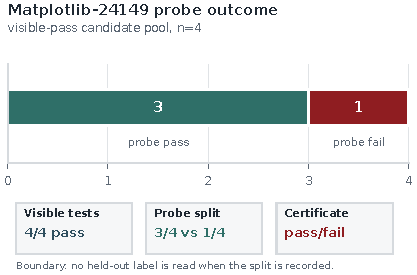
\includegraphics[width=\columnwidth]{figures/patchcourt_running_example_20260622.pdf}
  \caption{Quantitative running example for a full-package public probe. All four visible-passing candidates pass visible tests; the public probe splits them into three probe-pass candidates and one probe-fail candidate before any held-out label is read.}
  \Description{A Matplotlib public probe outcome chart: four visible-passing candidates enter, three pass the public probe, one fails it, and the certificate is marked as a pass/fail behavior split rather than a correctness oracle.}
\label{fig:running-example}
\end{figure}

\section{PatchCourt}

\subsection{Overview}

\patchcourt is a measurement and audit protocol for visible-passing repository patches.
Figure~\ref{fig:pipeline} shows the main flow with the counted objects at each stage: candidate sources produce patches, visible tests define the accepted-looking pool, public probes measure behavior before freeze, the certificate index is audited and frozen, and held-out labels are read only afterward.
The output is an evidence ledger whose rows bind a task, candidate source, probe layer, behavior signature, audit label, and calibration outcome.
Figure~\ref{fig:structured-patch-record} instantiates the record type behind the main result: visible-test pass is the acceptance gate, public-probe disagreement supplies pre-freeze evidence, and held-out calibration names the false-acceptance outcome.

\begin{figure}[t]
\begin{lstlisting}[style=patchcourtpatch]
[
 {"claim": "visible_pass_is_not_oracle",
  "task": "Matplotlib-24149", "case": "all-NaN bar",
  "edit": {"file": "lib/matplotlib/axes/_axes.py",
           "change": "guard all-NaN bar path"},
  "accepted_by": {"visible_tests": "pass"},
  "pre_freeze": {"probe": "full-package public probe",
                 "split": "3 preserve NaN bar / 1 axes failure",
                 "certificate": "pass_fail_bdc"},
  "audit": {"retain": true, "risk": "specification_debt"},
  "post_freeze": {"held_out": "fail",
                  "outcome": "false_acceptance"},
  "review_action": "inspect_or_rerank_before_accept"}
]
\end{lstlisting}
  \caption{Core PatchCourt record for false acceptance. A visible-passing Matplotlib edit reaches the acceptance gate, a public full-package probe splits candidate behavior before freeze, audit retains the record as specification-debt evidence, and post-freeze calibration marks the accepted-looking case as false acceptance.}
  \Description{JSON-like PatchCourt record for the Matplotlib all-NaN bar-plot case. It names the visible-pass-is-not-oracle claim, visible-test pass status, pre-freeze public-probe split, retained specification-debt audit label, post-freeze held-out failure, and the recommended inspect-or-rerank action.}
  \label{fig:structured-patch-record}
\end{figure}

\begin{figure*}[t]
  \centering
  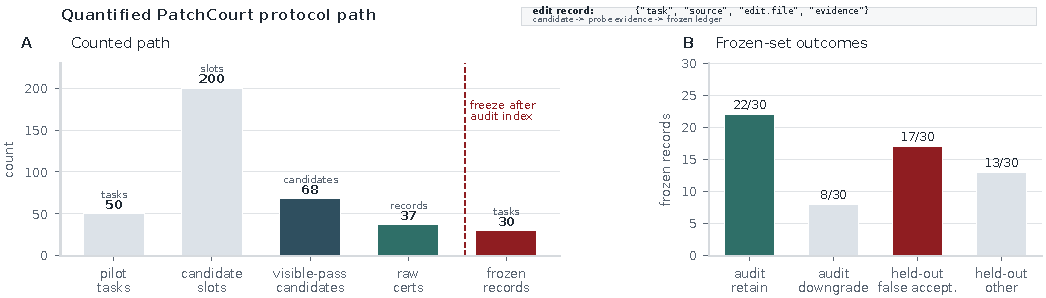
\includegraphics[width=\textwidth]{figures/patchcourt_main_pipeline_20260622.pdf}
  \caption{Quantified \patchcourt protocol path with structured-edit strip. The left panel counts pilot tasks, candidate slots, visible-pass candidates, raw certificates, and frozen records; the right panel shows frozen-set audit and held-out outcome counts.}
  \Description{Quantitative protocol figure: bar chart of the counted path from 50 pilot tasks through 200 candidate slots, 68 visible-pass candidates, 37 raw certificates, and 30 frozen records; bar chart of audit and held-out outcomes over the frozen set; compact JSON-like structured edit record inset.}
  \label{fig:pipeline}
\end{figure*}

\subsection{The Gold Boundary Principle}

Each task contains a public repository snapshot, public issue text, visible commands, and optional public snippets or reproducer fragments.
Evaluation-only fields are excluded before freeze: developer patch, test patch, FAIL\_TO\_PASS labels, PASS\_TO\_PASS labels, and held-out outcomes.
This boundary is the central design principle.
The pre-freeze protocol may observe only information that an acceptance-time auditor could obtain without opening the benchmark answer key.
The post-freeze phase then asks how often the frozen pre-freeze evidence coincides with held-out failure.
Keeping those phases separate lets the paper study acceptance risk without converting public probes into hidden labels.

\subsection{Inputs and Evidence Model}

For task $i$, let $R_i$ denote the repository snapshot, $I_i$ the public issue context, $V_i$ the visible command set, $P_i$ the generated patch candidates, $Q_i$ the public probe set, and $H_i$ the held-out calibration layer.
All pre-freeze evidence is a function of public inputs and candidate behavior:
\begin{equation}
\Omega_i^{\mathrm{pre}} = R_i \cup I_i \cup V_i \cup P_i \cup Q_i,
\qquad
\Omega_i^{\mathrm{pre}} \cap H_i = \varnothing .
\end{equation}
The freeze operator therefore selects records from pre-freeze evidence alone:
\begin{equation}
F(E^{\mathrm{pre}}, H) = F(E^{\mathrm{pre}}).
\end{equation}
For a candidate patch $p \in P_i$, the visible-passing candidate set is
\begin{equation}
C_i = \{p \in P_i : \mathrm{apply}_i(p)=1 \land \mathrm{visible}_i(p)=1\}.
\end{equation}
A public probe $q$ produces a normalized behavior signature
\begin{equation}
\sigma_i(p,q)=\mathcal{N}(\mathrm{run}(q, R_i \oplus p)),
\end{equation}
where normalization removes local path and formatting noise but preserves pass/fail outcomes, exceptions, assertions, API-visible values, and timeouts.
A behavioral-disagreement certificate exists when one admissible public probe separates visible-passing candidates into at least two behavior classes:
\begin{equation}
\begin{aligned}
\mathrm{BDC}_i(q)=\mathbf{1}\{&
q \in Q_i,\; \mathrm{goldblind}_i(q)=1,\\
&\left|\{\sigma_i(p,q):p\in C_i\}\right|\ge 2\}.
\end{aligned}
\end{equation}
The pass/fail subtype requires at least one passing and one failing signature among visible-passing candidates.
After the audit index is frozen, the selected calibration candidate $s_i \in C_i$ is evaluated against held-out labels, and false acceptance is measured as
\begin{equation}
\mathrm{FA}_i=
\mathbf{1}\!\left[s_i\in C_i \land
\exists h\in H_i:\sigma_i(s_i,h)=\mathrm{fail}\right].
\end{equation}
The primary estimand is conditional on the selected certificate-producing path:
\begin{equation}
\theta_S=\Pr(\mathrm{FA}_i=1\mid i\in S),\qquad
\widehat{\theta}_S=\frac{1}{|S|}\sum_{i\in S}\mathrm{FA}_i .
\end{equation}
This formalization treats a certificate as evidence of unresolved public behavior; patch correctness is resolved only by later calibration or external judgment.

\subsection{Candidate Generation and Visible Filtering}

\patchcourt ingests candidate diffs from multiple lanes.
Main evidence uses two recorded candidate-source lanes: an interactive model-generated lane and a project-controlled batch lane.
Inspection provenance is preserved in the artifact; both lanes are treated as project-controlled sources rather than independently authenticated external-model baselines.
The independent-source stress test uses a locally served Qwen2.5-Coder model with structured search/replace generation.
Table~\ref{tab:candidate-provenance} records the source provenance used by the paper-facing claims.

\begin{table*}[t]
\caption{Candidate-source provenance for paper-facing claims.}
\label{tab:candidate-provenance}
\centering
\scriptsize
\begin{tabularx}{\textwidth}{p{0.24\textwidth}rXX}
\toprule
Lane & Frozen & Candidate evidence & Scope \\
\midrule
Interactive model-generated lane & 7 & Model patch evidence; thirteen certificates before conservative deduplication. & Project-controlled candidate source used for the selected path. \\
Project-controlled batch lane & 23 & Calibration diversity with source provenance preserved in the artifact. & Main selected-path source; external-model independence is not attributed to this lane. \\
Open-source Qwen stress lane & 0 & Structured multi-sample edits yield visible-pass candidates and disagreement evidence. & Separate non-Codex stress test reported outside the frozen 30. \\
\bottomrule
\end{tabularx}
\end{table*}

Candidates are applied in isolated worktrees.
Environment routing is per task because repository-level benchmarks include old Python runtimes, compiled extensions, generated version files, and package-specific test entry points.
\patchcourt records apply status, visible status, execution-route metadata, compact outcome summaries, and candidate-source provenance.

\subsection{Probe Layers}

\patchcourt separates probe evidence into five layers:
\emph{source-isolated templates}, which are cheap discovery checks when full package execution is blocked;
\emph{issue-code probes}, which run executable public issue snippets;
\emph{full-package issue probes}, which import and drive the repository package around issue behavior;
\emph{package-integrity probes}, which test import or core API preservation; and
\emph{held-out calibration}, which runs evaluation-only labels after freeze.

This layering keeps each observation tied to the behavior it actually exercises.
Package-integrity splits describe import or API regression risk; issue correctness requires issue-code, full-package issue probes, or held-out calibration.
All-fail divergences are recorded separately from pass/fail behavioral certificates.
Held-out failures enter only after the audit index is frozen.
Post-disagreement overlays strengthen execution of already identified public behavior surfaces; they remain gold-blind and are reported as selected upgrade evidence.
Table~\ref{tab:probe-provenance} makes the probe provenance explicit, and Figure~\ref{fig:probe-code-cards} gives compact code-facing examples for an issue-code probe and an independent-source stress probe.

\begin{table}[t]
\caption{Probe provenance and timing. Held-out labels are read only after freeze.}
\label{tab:probe-provenance}
\centering
\scriptsize
\begin{tabularx}{\columnwidth}{lXX}
\toprule
Layer & Timing & Role and scope \\
\midrule
Source-isolated & Post-issue and pre-held-out; often after candidate-context materialization, before calibration labels. & Discovery/spec-debt signal only; cheap and issue-facing but not package behavior. \\
Issue-code & Public snippet exists pre-candidate; adaptation/routing may be post-disagreement, still gold-blind. & Stronger issue-tied evidence; selected overlays remain subset evidence. \\
Full-package & Mostly post-disagreement audit-upgrade overlay for selected targets, before label reading. & Main robustness check for selected certificates, not an unbiased discovery denominator. \\
Integrity & Post-Qwen visible-pass layer. & Regression/API-preservation evidence. \\
Held-out & After the frozen index is written. & Calibration label, never pre-freeze probe. \\
\bottomrule
\end{tabularx}
\end{table}

\begin{figure*}[t]
\begin{minipage}[t]{0.49\textwidth}
\begin{lstlisting}[style=patchcourtpatch]
# SymPy-23117 issue-code reproducer
from sympy import Array
a = Array([])
print("array", list(a))
print("shape", a.shape)

A/B/C: pass -> array []; shape (0,)
D:     fail -> empty-shape ValueError
\end{lstlisting}
\end{minipage}\hfill
\begin{minipage}[t]{0.49\textwidth}
\begin{lstlisting}[style=patchcourtpatch]
# Seaborn-3407 Qwen stress probe
probe: pairplot MultiIndex reproducer

qwen sample q0:
  pass -> axes_shape (4, 4)
qwen samples q1..q4:
  fail -> import or indexing path

scope: one issue-specific Qwen BDC
\end{lstlisting}
\end{minipage}
  \caption{Representative code-facing public probes. Left: an issue-code SymPy reproducer separates three passing candidates from one failing candidate. Right: the strongest Qwen issue-specific stress case separates one visible-pass sample that completes the public Seaborn reproducer from four visible-pass samples that fail.}
  \Description{Two code-like probe panels. The SymPy panel constructs an empty Array and records three passing candidates and one empty-shape failure. The Seaborn panel records one Qwen sample passing with axes shape 4 by 4 and four Qwen samples failing through import or indexing paths.}
  \label{fig:probe-code-cards}
\end{figure*}

\subsection{Behavior Signatures and Certificates}

Probe executions are normalized into behavior summaries: which candidate and public probe were checked, whether the probe passed, failed, or timed out, and a compact behavioral fingerprint.
A \bdc is emitted when visible-passing candidates for the same task and probe produce at least two behavior groups.
The strongest \bdcs have a pass/fail split on issue-related probes.
All-fail behavioral divergences are diagnostic and reported separately.

\subsection{Audit, Freeze, and Triage}

\patchcourt freezes a conservative certificate index before reading held-out labels.
The frozen set contains 30 task-level certificates.
Certificate audit labels each record as retain, downgrade, or reject; the frozen pass yields 22 retain, 8 downgrade, and 0 reject.
After freeze, \patchcourt runs held-out FAIL\_TO\_PASS calibration and records false acceptance.
This structured pass covers the 30 conservative records and occurs before held-out labels are read.
It was not blind to probe layer or candidate source, because those fields determine the evidence boundary; it was blind to held-out outcomes.
Inter-rater reliability is therefore outside the claim.
The artifact instead exposes stable certificate links, pass/fail behavior, audit rationales, downgrade reasons, and selected calibration candidates.
The rubric is deliberately conservative:
retain means that the probe is issue-relevant or strongly issue-adjacent, gold-blind, visible-pass-backed, and behaviorally meaningful;
downgrade means that the certificate remains useful but has a source-isolated, all-fail, routing, or missing-full-package caveat;
reject means that the record is not issue-relevant, not reproducible, not gold-blind, or not backed by visible-pass candidates.
No record in the frozen 30 was rejected because the freeze input had already filtered to conservative pass/fail records; weaker surviving cases were marked as downgrades rather than silently dropped.
Examples make the single-pass audit inspectable: retained Matplotlib and Seaborn records expose issue/full-package pass/fail behavior on visible-pass candidates, while downgraded Matplotlib and Sphinx records stay in the index with source-isolated, routing, or missing-upgrade caveats.

\patchcourt computes candidate-conditional oracle-gap lower bound (\ccogb), a specification-debt indicator, audit-weighted risk, and abstention rules.
\ccogb is reported as a lower-bound signal rather than a correctness probability.
It summarizes unresolved behavior mass within the accepted candidate pool.
Specification debt records reasons to keep a certificate under review, such as source-isolated status, downgraded audit, missing full-package validation, or all-fail divergence.

\subsection{The Freeze-and-Calibrate Protocol}

The empirical denominator is produced by this protocol, not chosen after calibration.
\patchcourt begins from a 50-task pilot and admits a paper-facing record only when four conditions hold: at least one visible-pass candidate exists; a gold-blind public probe separates visible-pass candidates; the audit record can be traced to a task, probe, source lane, and route; and the selected calibration candidate can be executed after freeze.
This yields 30 task-level records in the conservative certificate-producing path.
The choice favors fully auditable rows over prevalence coverage: every row has a certificate, probe provenance, candidate-source provenance, audit status, route record, selected candidate, and held-out outcome.
The paper therefore reports Wilson intervals and treats $\widehat{\theta}_S$ as a selected-path estimand rather than a population-wide SWE-bench rate.

\section{Research Questions and Setup}

\textbf{RQ1.} How often do visible/probe-accepted candidates become false acceptances under post-freeze held-out calibration?

\textbf{RQ2.} How much certificate evidence survives stronger issue-code or full-package probes?

\textbf{RQ3 (triage calibration).} Do pre-freeze signals provide calibrated triage, or only exploratory review cues?

\textbf{RQ4 (independent-source stress test).} What does a real independent Qwen source reveal about the supported scope of the evidence?

\subsection{Dataset and Freeze}

The selected-path study uses a frozen 30-certificate audit set built from a 50-task SWE-bench-style pilot.
The pilot was selected to stress repository-level repair conditions that matter for acceptance audit: visible commands, real package environments, issue text, candidate patches, and executable public probes.
From that pilot, the paper-facing denominator keeps only conservative task-level records that pass the freeze-and-calibrate protocol described above.
This choice is deliberate.
It makes each row checkable enough for an ICSE artifact review, while keeping the rate tied to the selected certificate-producing path.

The unit of analysis is one frozen task-level certificate record, not an individual model sample, repository family, or benchmark issue pool.
Each record stores the task, public probe, selected candidate, source lane, evidence layer, audit status, routing summary, and post-freeze held-out outcome.
When several candidate disagreements exist for a task, the audit index deduplicates to one conservative paper-facing record using a fixed precedence: pass/fail certificates over all-fail divergences, stronger public execution layers over weaker source-isolated layers when available at freeze time, retain over downgrade, and stable record order as the final tie-breaker.
The held-out calibration candidate is not chosen after seeing held-out labels.
It is the probe-passing visible-pass candidate selected by the frozen record, preferring model-generated patches over no-op controls and then the deterministic record order.
All 30 stored calibration candidates pass their pre-freeze probe.
The freeze point is the creation of the frozen certificate index; held-out calibration reads evaluation-only labels only afterward.
Figure~\ref{fig:selection-funnel} shows the denominator, audit, and calibration splits that define the selected path.
The anonymous artifact includes the full numeric funnel and a 50-task pilot drop-reason table that records which pilot tasks entered the frozen 30, which broad all-fail record was excluded, and which tasks did not produce conservative paper-facing certificates.
The study therefore answers a conditional question: among auditable visible-pass cases that already show public behavioral disagreement, how often does acceptance fail when the held-out layer is finally opened?

\begin{figure*}[t]
  \centering
  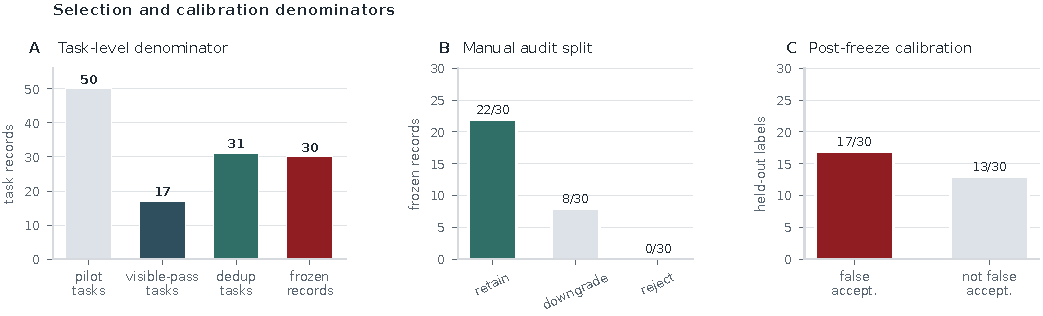
\includegraphics[width=\textwidth]{figures/patchcourt_selection_funnel_20260622.pdf}
  \caption{Selection and calibration denominators for the selected certificate-producing path. The panels separate task-level selection counts, manual audit labels, and post-freeze held-out labels so the `17/30' result remains tied to the frozen record set.}
  \Description{Three-panel denominator figure: task-level bars for 50 pilot tasks, 17 visible-pass tasks, 31 deduplicated tasks, and 30 frozen records; audit bars for 22 retain, 8 downgrade, and 0 reject labels; held-out bars for 17 false acceptances and 13 other records.}
  \label{fig:selection-funnel}
\end{figure*}

Table~\ref{tab:route-stability} records where routing changed executability.
The frozen certificate index itself did not change after labels were read; routing changes are append-only execution repairs or stronger-probe overlays.

\begin{table}[t]
\caption{Route-stability controls. Routing repairs improve executability and stronger-probe coverage without rewriting the frozen certificate index.}
\label{tab:route-stability}
\centering
\footnotesize
\begin{tabularx}{\columnwidth}{XXX}
\toprule
Layer & Before routing repair & Paper-facing use \\
\midrule
Held-out FAIL\_TO\_PASS & 15/30 executable & 30/30 executable in Table~\ref{tab:heldout}. \\
Main probe upgrades & 2/10 upgraded BDC targets & 6/10 pass/fail full-package or issue-code BDC targets. \\
Frozen audit index & 30 conservative records & Unchanged source of truth for calibration. \\
Independent-source gate & Qwen stress lane only & Batch candidates remain project-controlled rather than an external-model baseline. \\
\bottomrule
\end{tabularx}
\end{table}

\begin{table}[t]
\caption{Cost and overhead summary for the paper-facing layers. The table reports work units and execution counts rather than machine-specific wall-clock minutiae.}
\label{tab:overhead}
\centering
\scriptsize
\begin{tabularx}{\columnwidth}{XrX}
\toprule
Item & Value & Note \\
\midrule
Candidate slots per pilot task & 4.0 & Three non-control slots plus one no-op control. \\
Candidate-probe executions & 148 & 37 certificate records times four candidate versions. \\
Main upgrade probe runs & 40 & 10 targets times four candidate versions. \\
Extra full-package probe runs & 40 & 10 targets times four candidate versions. \\
Held-out calibration runs & 30 & Executed after freeze; all records executable. \\
Certificate-audit work units & 30 & Single structured audit pass; minutes not logged. \\
Route blockers before / after repair & 15/30 to 0/30 & Held-out unavailable records before and after routing. \\
Upgrade non-BDC targets before / after repair & 8/10 to 4/10 & Remaining failures are old-dependency, all-pass, or all-fail candidate-pool limits. \\
\bottomrule
\end{tabularx}
\end{table}

\subsection{Metrics and Statistical Treatment}

We report held-out executability, held-out false-acceptance count and Wilson interval, specification-debt count, pass/fail BDC yield under upgraded probes, correlation and rerank scores, abstention coverage, and independent-source applicability.
All primary proportions use Wilson 95\% intervals.
For RQ3, random-review precision uses the hypergeometric baseline implied by 17 false acceptances among the 30 records in the selected certificate-producing path: expected precision is 0.567 at any fixed review budget, with central 95\% random intervals of [0.30, 0.80] at $k=10$ and [0.45, 0.70] at $k=20$.
Ranking and correlation results are therefore treated as preliminary triage evidence rather than calibrated prediction.

\section{Results}

Figure~\ref{fig:certificate-ladder} grounds the aggregate results in one quantified certificate-level case before the RQ-specific tables.
It shows the candidate-level public-probe split and the record-level held-out label without treating the certificate as a held-out label.

\begin{figure*}[t]
  \centering
  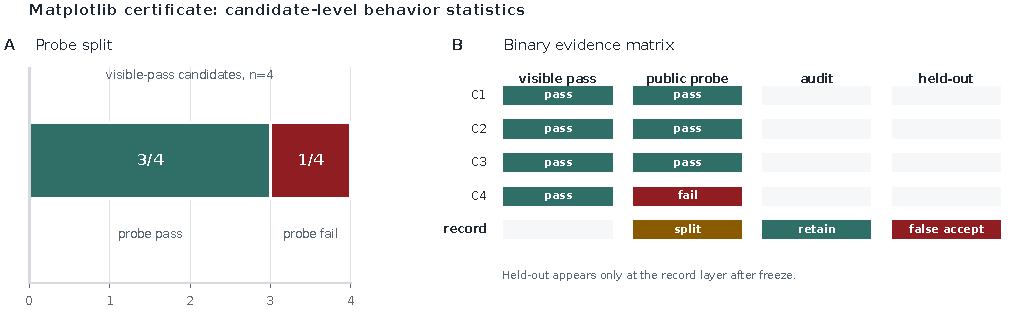
\includegraphics[width=\textwidth]{figures/patchcourt_certificate_evidence_ladder_20260622.pdf}
  \caption{Quantified certificate evidence for the Matplotlib all-NaN bar-plot case. The public probe splits four visible-passing candidates into three probe-pass and one probe-fail candidates; the record is retained before freeze and receives its false-acceptance label only after held-out calibration.}
  \Description{Two-panel certificate figure: a stacked bar showing three of four visible-passing candidates pass the public probe and one fails it; a binary evidence matrix showing visible pass, public-probe result, audit retain status, and post-freeze false-acceptance label.}
  \label{fig:certificate-ladder}
\end{figure*}

\subsection{RQ1: Held-Out False Acceptance}

Table~\ref{tab:heldout} summarizes the frozen calibration within the selected certificate-producing path.
All 30 frozen held-out calibrations execute.
Of these selected records, 17 are false acceptances under held-out FAIL\_TO\_PASS labels.
Specification debt is present in 26 of 30 cases.
False acceptance remains common after certificate audit: retained records have 13/22 false acceptances and downgraded records have 4/8.
Specification debt is a conservative high-coverage signal in this set: all 17 false acceptances are in the specification-debt-present stratum, while the four debt-absent records have zero false acceptances.

\begin{table}[t]
\caption{Frozen held-out calibration after the certificate index is frozen. The set is selected, not a SWE-bench population estimate.}
\label{tab:heldout}
\centering
\begin{tabular}{lr}
\toprule
Quantity & Value \\
\midrule
Frozen conservative certificates & 30 \\
Certificate audit retain/downgrade/reject & 22/8/0 \\
Held-out executable tasks & 30/30 \\
Selected-path false acceptances & 17/30 \\
Wilson 95\% CI for false acceptance & [0.392, 0.726] \\
Specification-debt signal & 26/30 \\
Wilson 95\% CI for specification debt & [0.703, 0.947] \\
\midrule
Retain false-acceptance rate & 13/22 \\
Downgrade false-acceptance rate & 4/8 \\
Spec-debt-present false-acceptance rate & 17/26 \\
Spec-debt-absent false-acceptance rate & 0/4 \\
\bottomrule
\end{tabular}
\end{table}

\noindent\textbf{Finding 1.}
Table~\ref{tab:heldout} shows that visible/probe acceptance leaves substantial residual risk in the selected frozen audit set.
The claim is not that all visible-passing patches are wrong, but that visible/probe acceptance is an unsafe endpoint without additional audit evidence.

\subsection{RQ2: Stronger Probe Validation}

Table~\ref{tab:upgrades} reports both probe-upgrade layers.
The upgrade layer executes 40 probes across 10 high-signal targets.
Six targets yield pass/fail \bdcs under full-package or issue-code execution: Django empty sitemap last-modified, Django template join autoescape, Matplotlib all-NaN bar plot, Seaborn MultiIndex pairplot, Scikit-Learn LabelEncoder empty transform, and SymPy empty array.
An additional full-package layer over 10 targets yields seven BDC tasks, six of which are pass/fail and one of which is all-fail divergence.

\begin{table*}[t]
\caption{Probe-upgrade evidence. Stronger issue-code and full-package probes preserve pass/fail disagreement for selected targets; all-fail divergence is reported separately.}
\label{tab:upgrades}
\centering
\begin{tabularx}{\textwidth}{lrr>{\raggedright\arraybackslash}X}
\toprule
Layer & Targets & Pass/fail BDCs & Positive tasks / notes \\
\midrule
Main full-package or issue-code upgrades & 10 & 6 & Django-16255, Django-16873, Matplotlib-24149, Seaborn-3407, Scikit-Learn-10508, and SymPy-23117. Wilson 95\% CI: [0.313, 0.832]. \\
Extra full-package upgrades & 10 & 6 & Seven total BDC tasks; six pass/fail and one all-fail divergence. This layer strengthens package-level robustness without being merged into the main issue-specific count. \\
Qwen issue/full-package probes & 11 visible-pass tasks & 1 & Seaborn-3407 is the only Qwen issue-specific pass/fail BDC after multi-sample generation and rescue. \\
Qwen package-integrity probes & 11 visible-pass tasks & 4 & Integrity positives for Seaborn, Flask, and Scikit-Learn expose full-package regression risk. \\
\bottomrule
\end{tabularx}
\end{table*}

\noindent\textbf{Finding 2.}
Table~\ref{tab:upgrades} shows that selected certificates can survive issue-code and full-package upgrades, extending the evidence beyond source-isolated templates.
However, upgrade results remain a selected subset, and all-fail divergence must remain separate from pass/fail BDC counts.

\subsection{RQ3 Triage Signals}

Table~\ref{tab:triage} shows that raw \ccogb alone is under-calibrated in the frozen 30-task table.
Specification debt and audit-weighted risk provide modest review-budget signals: audit-weighted risk increases precision@10 from 0.400 to 0.600 and precision@20 from 0.550 to 0.650 relative to raw \ccogb.
Against a random-review baseline, however, these values remain inside the finite-sample random intervals, so the evidence justifies triage exploration rather than a calibrated ranking claim.
The specification-debt abstention rule is conservative and high coverage: it abstains on 26/30 tasks and captures all 17 false acceptances in the selected certificate-producing path.
Such a rule is too broad to be a production policy by itself, but it usefully shows that the ledger can drive explicit risk-control decisions.

\begin{table}[t]
\caption{Triage and abstention. Random review has expected P@10/P@20 of 0.567/0.567; central 95\% random intervals are [0.30, 0.80] at $k=10$ and [0.45, 0.70] at $k=20$.}
\label{tab:triage}
\centering
\footnotesize
\begin{tabularx}{\columnwidth}{Xrrr}
\toprule
Signal & Pearson & AP & P@10/P@20 \\
\midrule
Raw \ccogb & -0.116 & 0.557 & 0.400 / 0.550 \\
\ccogb + spec debt & 0.146 & 0.612 & 0.500 / 0.650 \\
Audit-weighted risk & 0.129 & 0.617 & 0.600 / 0.650 \\
Spec-debt indicator & 0.449 & 0.612 & -- \\
Random review order & -- & -- & 0.567 / 0.567 \\
\midrule
Abstention rule & Rate & Capture & Residual FA \\
\midrule
\ccogb $\ge 0.50$ & 0.167 & 0.118 & 0.600 \\
\ccogb $\ge 0.75$ & 0.067 & 0.059 & 0.571 \\
Specification debt & 0.867 & 1.000 & 0.000 \\
\bottomrule
\end{tabularx}
\end{table}

\noindent\textbf{Finding 3.}
Table~\ref{tab:triage} reads as a small-sample calibration result.
Specification debt is conservative and high coverage, while the broad abstention rate and random-order intervals keep raw disagreement scores in the category of review cues at this sample size.

\subsection{Independent Qwen Stress Test}

The independent-source experiment asks how far the evidence pipeline carries when candidate patches come from a truly non-Codex local model source.

Naive diff generation with Qwen rarely reaches the apply-and-visible-pass gate in a form that can yield certificate evidence.
Structured search/replace generation improves applicability and creates a visible-pass stress pool.
On the frozen set, structured generation yields applyable candidates for 17 tasks and visible-pass candidates for 11 tasks.
Multi-sample generation over those visible-pass tasks produces a larger candidate pool, but issue-specific pass/fail disagreement remains rare.

Table~\ref{tab:claim-boundary} summarizes the supported inference for each evidence type.
This lane is a partial-positive stress test: \patchcourt ingests a real non-Codex source and finds nonzero disagreement, while broad issue-specific reproduction remains unsupported by the observed yield.
Figure~\ref{fig:probe-code-cards} shows the strongest issue-specific Qwen case as a code-facing public probe and normalized output split.

\begin{table*}[t]
\caption{Evidence scope by result type. Each row states the inference supported by the evidence and the main limit on interpretation.}
\label{tab:claim-boundary}
\centering
\begin{tabularx}{\textwidth}{lXX}
\toprule
Evidence type & Supported inference & Main limit \\
\midrule
Frozen held-out calibration (17/30 false acceptance; 26/30 spec debt) & Visible/probe acceptance often fails held-out labels in the selected certificate-producing path. & Selected-path rate, not a SWE-bench-wide population estimate or patch-correctness judgment. \\
Main and extra probe upgrades (6/10 and 6/10 pass/fail) & Stronger full-package or issue-code probes preserve disagreement for selected targets. & Evidence for selected targets rather than a calibrated predictor for every task. \\
Qwen issue-specific pass/fail BDC (1 task) & A single independent-source issue-specific compatibility case; strongest case is Seaborn MultiIndex pairplot. & Limited yield, so broad Qwen reproduction remains unsupported. \\
Qwen package-integrity BDCs (4 tasks) & Independent-source visible-pass patches can break or preserve full-package behavior differently. & Integrity/regression evidence rather than issue-correctness evidence. \\
Qwen all-fail divergences and rescue negatives & Diagnostic behavior diversity and a documented negative result. & No added positive pass/fail BDC yield. \\
\bottomrule
\end{tabularx}
\end{table*}

\noindent\textbf{Qwen scope.}
Structured generation turns an applicability failure into a visible-pass multi-sample pool.
The retained evidence consists of one issue-specific pass/fail certificate and four package-integrity certificates.
Raw generation and applicability counts are preserved in the artifact rather than treated as main-paper claims.

Figure~\ref{fig:quant-summary} consolidates the main result denominators after the RQ-specific tables.
Panel A shows the selected-path calibration rates and Wilson intervals.
Panel B separates pass/fail upgrade yield from other disagreement and no-BDC outcomes.
Panel C records the routing repairs that made calibration and upgrade execution complete enough for the paper-facing tables.
Panel D shows why reranking remains a boundary analysis: the best review cue improves over raw \ccogb, but the finite-sample random baseline remains close.
The artifact contains the corresponding single-purpose plots for calibration rates, probe-upgrade yield, source/layer mix, route stability, rerank/abstain, Qwen yield, and repository-level outcome distribution.

\begin{figure*}[t]
  \centering
  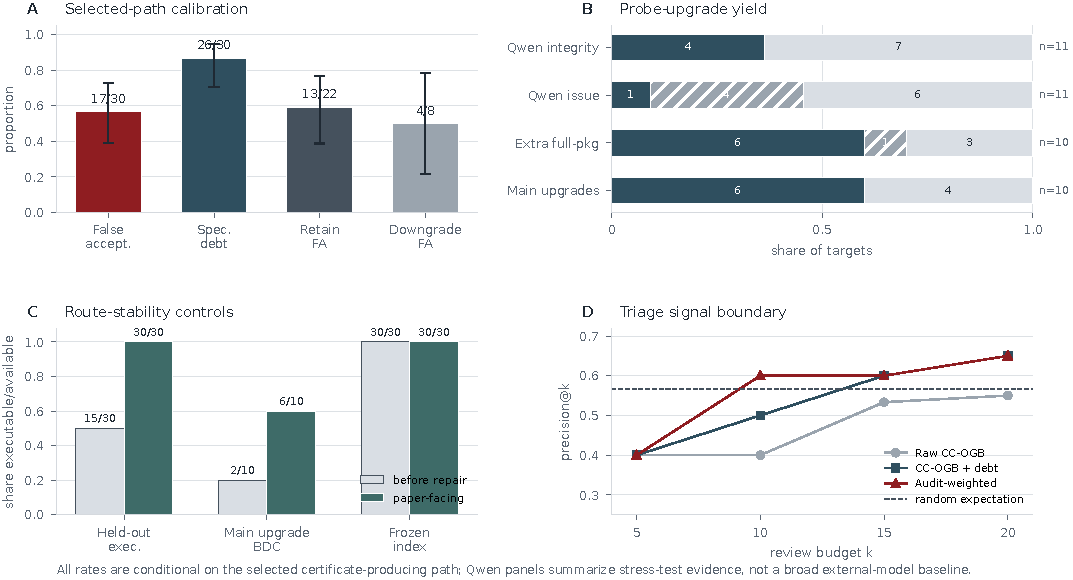
\includegraphics[width=\textwidth]{figures/patchcourt_quantitative_summary_20260622.pdf}
  \caption{Quantitative result summary. Panel A reports selected-path calibration rates with Wilson 95\% intervals. Panel B reports pass/fail BDC yield by probe layer and keeps Qwen issue and integrity evidence separated. Panel C shows routing repairs without changing the frozen audit index. Panel D summarizes rerank precision as boundary evidence rather than a calibrated predictor.}
  \Description{Four-panel quantitative summary: selected-path calibration bars with confidence intervals; probe-upgrade stacked yield bars; route-stability before and after bars; and triage precision lines against a random-review expectation.}
  \label{fig:quant-summary}
\end{figure*}

\section{Qualitative Cases}

The following cases ground the aggregate tables in certificate-level evidence.
They connect the table-level claims in Tables~\ref{tab:heldout}--\ref{tab:claim-boundary} to artifact audit rows.
Each case links to the underlying certificate and table row for inspection.
Code-facing evidence appears in Figures~\ref{fig:structured-patch-record}, \ref{fig:probe-code-cards}, and \ref{fig:django-code-card}.

\subsection{Seaborn MultiIndex Pairplot}

Seaborn-3407 is the strongest cross-source case.
It appears in the main upgraded probe layer and is also the only Qwen issue/full-package pass/fail BDC after multi-sample generation.
The issue-level package probe separates visible-passing edits: the main lane reports three pass and one fail, and the Qwen lane reports one pass and four fail, with the passing group constructing the 4-by-4 axes grid in Figure~\ref{fig:probe-code-cards}.
The certificate supports independent-source compatibility without carrying a broad Qwen reproduction claim.

\subsection{Matplotlib All-NaN Bar Plot}

Matplotlib-24149 links a full-package upgraded probe to a post-freeze held-out false acceptance.
Visible tests accept candidates that differ on an all-NaN plotting edge case.
After routing repair, the package-level probe records three pass, one fail, and no timeouts: the passing group preserves one bar with a NaN coordinate, while the failing group exits through the Matplotlib axes stack.
The certificate localizes the behavioral split; the false-acceptance label comes only from later frozen held-out calibration.

\subsection{Scikit-Learn LabelEncoder Empty Transform}

Scikit-Learn-10508 separates issue behavior from package-integrity risk.
In the main lane, the LabelEncoder empty-transform reproducer yields a pass/fail certificate once compiled-extension/build routing is repaired.
The record has three pass, one fail, and no timeouts: the passing group preserves an empty one-dimensional output, while the failing group hits a NumPy casting path.
In the Qwen lane, issue-specific probes remain all-fail, while a package-integrity probe reports two pass and three fail on whether LabelEncoder can be imported and constructed; \patchcourt treats that split as package-risk evidence rather than issue-correctness evidence.

\subsection{Django Semantic Split}

Django-16873 is a full-package semantic split under template rendering with autoescape disabled.
The record has three pass, one fail, and no timeouts: the passing group preserves literal line-break separators, while the failing group escapes them and raises an assertion.
The later held-out label is not false acceptance, so the case shows how \bdcs flag unresolved semantics without becoming hidden-test labels.

\begin{figure}[t]
\begin{lstlisting}[style=patchcourtpatch]
# Django-16873 full-package public probe
out = render_join(autoescape=False)

A/B/C: pass -> "alpha\nbeta"
D:     fail -> escaped separator assertion

certificate: pass/fail BDC before freeze
boundary: semantic split, not hidden-test oracle
\end{lstlisting}
  \caption{Code-facing Django case probe. The public full-package probe splits three visible-passing candidates that preserve separator behavior from one that escapes it.}
  \Description{A compact code-like Django probe card showing render_join with autoescape disabled, three passing candidates preserving alpha newline beta, one failing candidate with an escaped separator assertion, and a boundary note that the certificate is not a hidden-test oracle.}
  \label{fig:django-code-card}
\end{figure}

\subsection{SymPy Issue-Code Layer}

SymPy task 23117 demonstrates the issue-code layer.
The public snippet in Figure~\ref{fig:probe-code-cards} yields three pass, one fail, and no timeouts, with the passing group preserving an empty array result.
This issue-tied layer is stronger than a source-isolated template while remaining separate from held-out calibration.

\section{Related Work}

\subsection{Repository-Level Repair, Agents, and Benchmarks}

Repository-level repair sits on benchmark and model infrastructure.
Defects4J, ManyBugs, Bugs.jar, Bears, BugsInPy, and QuixBugs established controlled real-bug substrates for repair and testing research \cite{just2014defects4j,le2015manybugs,saha2018bugsjar,madeiral2019bears,widyasari2020bugsinpy,lin2017quixbugs}.
SWE-bench and SWE-bench+ move the unit of work to GitHub issues and real repository snapshots \cite{jimenez2024swebench,aleithan2024swebenchplus}.
Code models and code benchmarks provide the upstream capability base for these systems \cite{feng2020codebert,lu2021codexglue,chen2021codex,austin2021program,wang2021codet5,li2022alphacode,nijkamp2023codegen,roziere2023codellama,guo2024deepseekcoder}.
Agent work studies repository search, tool use, turn management, and candidate-fix generation \cite{yang2024sweagent,zhang2024autocoderover,bouzenia2025repairagent,xia2024agentless,gao2026moreless,tian2026ensemble}.
\patchcourt enters after that generation process.
It audits the moment when a visible-pass candidate would otherwise be accepted and records what public evidence remains unresolved.

\subsection{LLM Repair and APR Overfitting}

Automated program repair has long separated test-passing plausibility from semantic correctness, across generate-and-validate, template, semantic, and learning-based repair \cite{weimer2009genprog,legoues2012systematic,kim2013par,nguyen2013semfix,long2016prophet,mechtaev2016angelix,xuan2017nopol,tufano2019learning,lutellier2020coconut,jiang2021cure,zhu2021recoder,xia2022less,xia2023conversational}.
Patch plausibility and overfitting studies show why passing tests can be insufficient \cite{qi2015plausibility,smith2015overfitting,ye2021automated,gazzola2019survey}.
Recent ICSE work revisits APR in the LLM era through code-language-model impact, bug-report/test coupling, objective alignment, input reduction, and unnaturalness-based ranking \cite{jiang2023impact,motwani2023better,xu2025aligning,yang2026inputreduction,yang2025unnaturalness}.
\patchcourt operationalizes a narrower acceptance-time question for repository-level LLM patch pools: after visible tests pass, can public, gold-blind behavior measurements expose an auditable risk record before benchmark labels are opened?

\subsection{Patch Correctness, Benchmark Validity, and Contamination}

Recent SWE-bench correctness work asks whether benchmark-accepted issues are genuinely fixed and uses PatchDiff to compare generated patches against human-written ground-truth patches \cite{wang2025swebenchcorrectness}.
Diagnostic benchmark work studies whether strong SWE-bench performance may reflect memorization or benchmark exposure rather than issue reasoning \cite{liang2025illusion,jain2025livecodebench}.
These studies challenge the meaning of a benchmark pass after evaluation.
\patchcourt instead freezes an evidence ledger before developer patches, hidden tests, or stronger labels enter the process, then uses held-out calibration to measure alignment with later failure.
The claim is weaker than retrospective correctness judgment, but it is available at the acceptance boundary.

\subsection{Generated Tests, Oracles, and Validation}

Generated tests can strengthen repair validation, but they face the test oracle problem: producing an input is easier than knowing the expected behavior.
Classic testing work developed feedback-directed random testing, symbolic execution, dynamic test generation, and mutation-analysis foundations for exposing untested behavior \cite{godefroid2005dart,sen2005cute,cadar2008klee,pacheco2007feedback,fraser2011evosuite,jia2011mutation}.
Search-based and LLM-based testing studies continue this line with generated tests, bug reproduction, and execution feedback \cite{lemieux2023codamosa,kang2023fewshot,chen2023codet,liu2023evalplus,ahmed2026heterogeneous,shin2026retrieval,li2026knowledge}.
Oracle-generation work, including TOGA, neural-oracle evaluations, and TOGLL, studies when automated or LLM-produced assertions become correct and strong enough for testing \cite{barr2015oracle,pezzezhang2014oracles,dinella2022toga,hossain2023neuraloracle,hossain2025togll}.
\patchcourt treats probes as evidence-producing instruments rather than as generated oracle labels.
Their evidentiary weight depends on the layer: source-isolated, issue-code, full-package issue, package-integrity, or post-freeze held-out calibration.

\section{Threats to Validity}

\textbf{Internal validity.}
Probe code may encode an incomplete interpretation of the issue.
Environment routing may introduce artifacts, especially for repositories with compiled extensions, old dependencies, or package-specific entry points.
\patchcourt mitigates this by logging route metadata, reporting route stability, and separating source-isolated, issue-code, full-package, package-integrity, and held-out layers.
The rubric still relies on human judgment; certificate links, pass/fail behavior, audit labels, and downgrade reasons are exposed in the artifact.

\textbf{Construct validity.}
\bdcs localize public behavioral disagreement, while \ccogb summarizes a candidate-conditional lower-bound signal.
All-fail divergence is weaker than pass/fail disagreement, and package-integrity probes measure regression or API preservation rather than issue behavior; the tables keep those evidence types separate.

\textbf{External validity.}
The main calibration set contains 30 frozen certificates selected through an audit pipeline.
The resulting rates describe this selected certificate-producing path.
Broader repository, language, and candidate-source coverage is needed before estimating field-wide behavior.
The selection funnel in Figure~\ref{fig:selection-funnel} is included to make this selected-set boundary explicit.

\textbf{Conclusion validity.}
The correlation, rerank, and abstain results are small-$N$ and preliminary.
Specification debt performs strongly in this table, but the pattern may reflect the selected certificate set.
The triage results are practical evidence for review prioritization rather than a validated predictor.

\textbf{Independent-source validity.}
One issue-specific pass/fail BDC and four package-integrity BDCs make the Qwen lane a stress test with limited issue-specific yield.
The direct-diff Qwen run remains a negative baseline, and the project-controlled batch lane remains separate from an authenticated external-model baseline.

\textbf{Gold-boundary validity.}
\patchcourt's strongest design claim is the pre-freeze/post-freeze separation.
The artifact must keep this separation inspectable.
If any future experiment uses developer patches, test patches, FAIL\_TO\_PASS, or PASS\_TO\_PASS before freeze, it must be excluded from the main gold-boundary claim.

\section{Artifact}

The anonymous artifact is designed for inspect-only reproduction first, with optional deeper replay where compute and model access are available.
At Level~0, reviewers inspect frozen tables, reports, certificates, and audit labels without external model access.
At Level~1, they run the packaged verifier to regenerate paper-facing summaries from the shipped CSV, JSONL, and Markdown files.
At Levels~2--3, they replay selected probes or regenerate candidates, visible tests, probes, BDCs, ledgers, and calibration with suitable runtimes and model access.

The bundle contains paper tables, result data files, frozen audit indices, Qwen audit reports, figure sources, rendered figures, and an anonymous claim-boundary card.
It excludes passwords, API keys, transient cookies, private keys, and author-identifying machine paths.
Execution identifiers remain inside index files for auditability, while the paper-facing text uses stable concepts.

\section{Discussion and Conclusion}

This paper studied a concrete failure mode in repository-level LLM repair: visible tests can accept patches that still encode unresolved issue behavior.
We characterize that gap as an acceptance-time measurement problem.
\patchcourt turns visible-passing patches into executable hypotheses, records public behavior disagreements before benchmark labels are read, and calibrates the frozen records after held-out labels become available.

The method follows a deliberately narrow flow.
Candidate patches first pass through repository apply and visible-test filters.
Public probes measure behavior at source-isolated, issue-code, full-package, and package-integrity layers.
Executions are normalized into behavior signatures and retained as certificate records when the audit rubric finds actionable disagreement.
After freeze, held-out calibration estimates how often the selected certificate-producing path corresponds to false acceptance or specification debt.

The main empirical result is that visible-pass acceptance is a poor stopping point on this selected path.
Among 30 frozen certificate-producing records, 17 become false acceptances under post-freeze held-out calibration and 26 retain specification-debt signals.
Stronger issue-code or full-package upgrades preserve pass/fail disagreement in 6/10 selected upgrades, and a separate package-level upgrade set preserves another 6/10 certificates.
The Qwen stress lane demonstrates source compatibility with one issue-specific and four package-integrity disagreement cases, while keeping the main claim anchored in the audited frozen path.

The broader implication is operational.
Visible tests should trigger inspection, reranking, or abstention when public executable evidence shows unresolved behavior; they should not be the final oracle for accepting repository-level repairs.
Future work should expand the selected path across more repositories and model sources, add multi-rater audit, and integrate certificate evidence into repair agents before deployment-time acceptance decisions.
\bibliographystyle{IEEEtran}
\bibliography{references}

\end{document}
